\subsection{Cantilever beam problem}\label{sec:cantilever}
Consider the cantilever beam problem shown in Figure \ref{fg:cantilever_model} with length $L = 48$, width $D = 12$, and the incompressible material parameters are employed with Young's modulus $E = 3\times 10^6$, Poisson's ratio $\nu = 0.5-10^{-8}$. The left hand side is fixed and the right side subject to a concentrated force $P = 1000$. All the prescribed values in the boundary conditions are evaluated by the analytical solution that is given as follows \cite{timoshenko1969}:
\begin{equation}
\left\{
\begin{aligned}
u_x(\boldsymbol{x}) &= - \frac{Py}{6\bar{E}I} \left( (6L - 3x)x + (2 + \bar{\nu})(y^2 - \frac{D^2}{4}) \right) \\
u_y(\boldsymbol{x}) &= \frac{P}{6\bar{E}I} \left( 3 \bar{\nu} y^2(L-x) + (4+5\bar{\nu}) \frac{D^2x}{4} + (3L-x)x^2 \right)
\end{aligned}
\right.
\end{equation}
where $I$ is the beam's moment of inertia, $\bar{E}$ and $\bar{\nu}$ are the material parameters for plane strain hypothesis, they can be expressed by:
\begin{equation}
I = \frac{D^3}{12}, \quad \bar{E} = \frac{E}{1-\nu^2}, \quad \bar{\nu} = \frac{\nu}{1-\nu}
\end{equation}
And correspondingly, the stress components are evaluated by
\begin{equation}
\left\{
\begin{aligned}
\sigma_{xx} &= - \frac{P(L-x)y}{I} \\
\sigma_{yy} &= 0 \\
\sigma_{xy} &= \frac{P}{2I}(\frac{D^2}{4}-y^2)
\end{aligned}
\right.
\end{equation}

\begin{figure}[H]
\centering
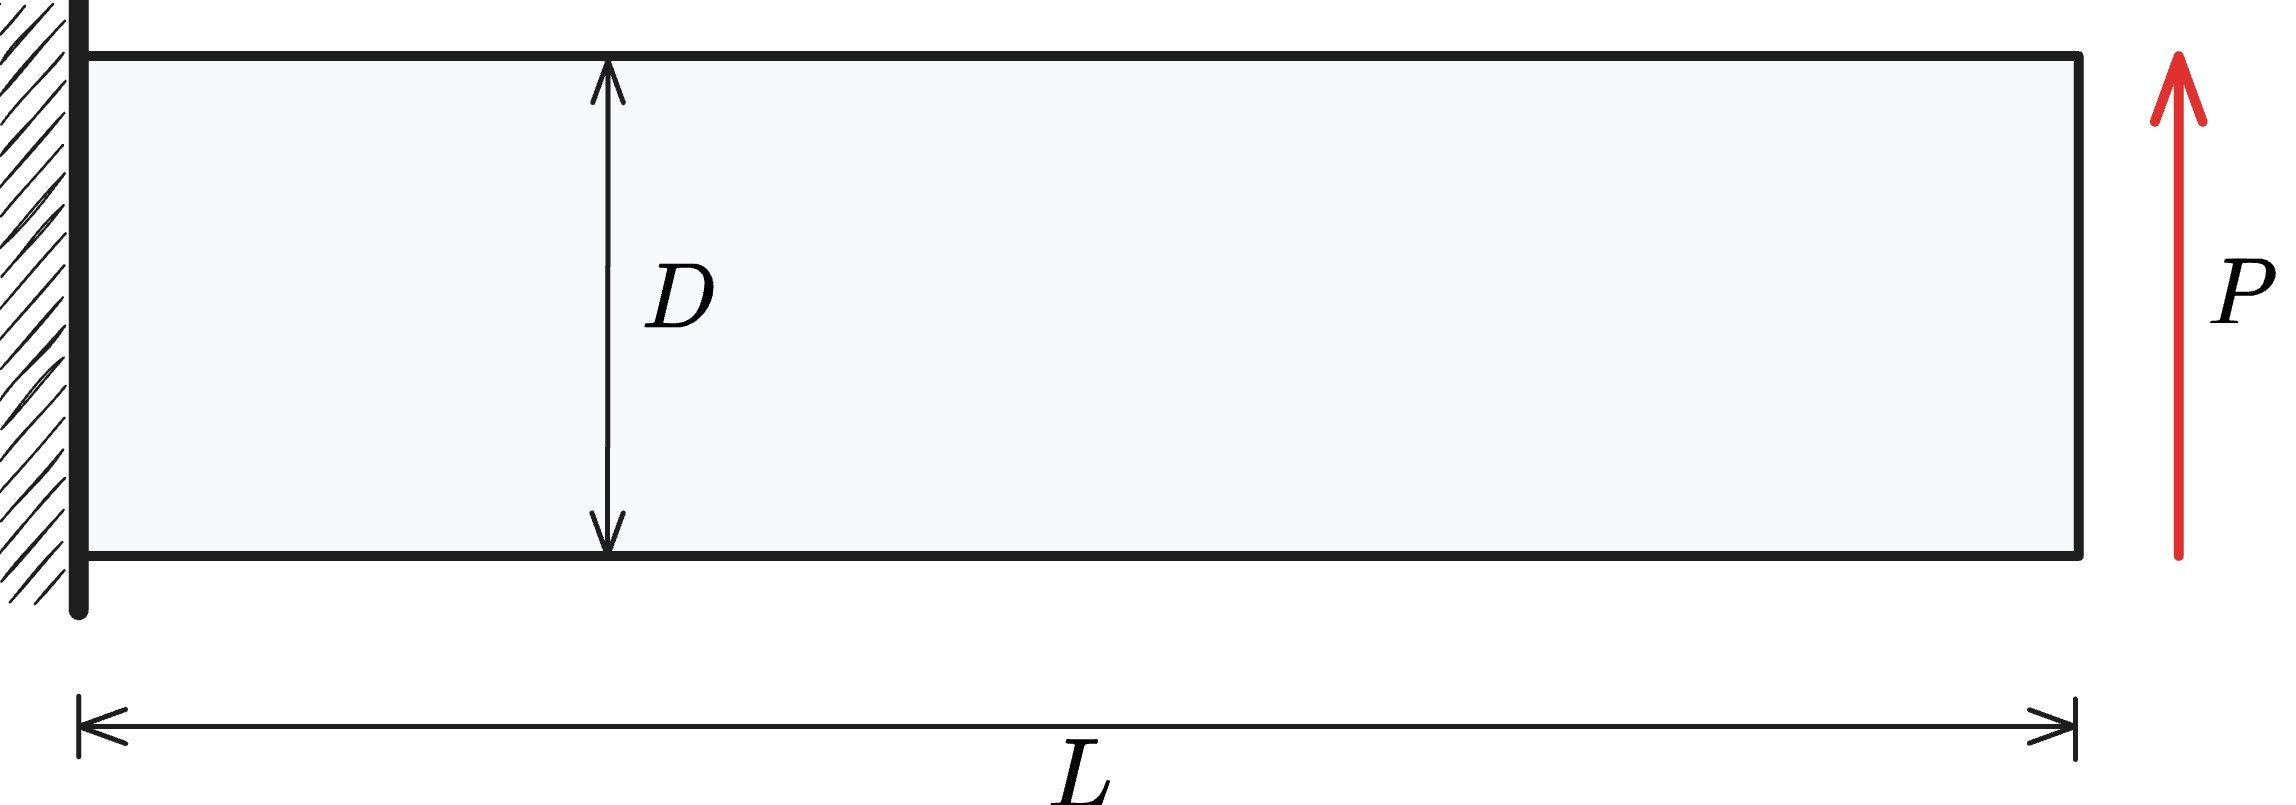
\includegraphics[width=0.7\textwidth]{cantilever_model.png}
\caption{Illustration of cantilever beam problem}\label{fg:cantilever_model}
\end{figure}

\begin{figure}[!hp]
\centering
\begin{subcaptiongroup}
\begin{tabular}{c@{\hspace{0pt}}c}
$\Vert \boldsymbol{u} - \boldsymbol{u}_h \Vert_V$ & $\Vert p - p_h \Vert_Q$ \\
\raisebox{-0.8\height}{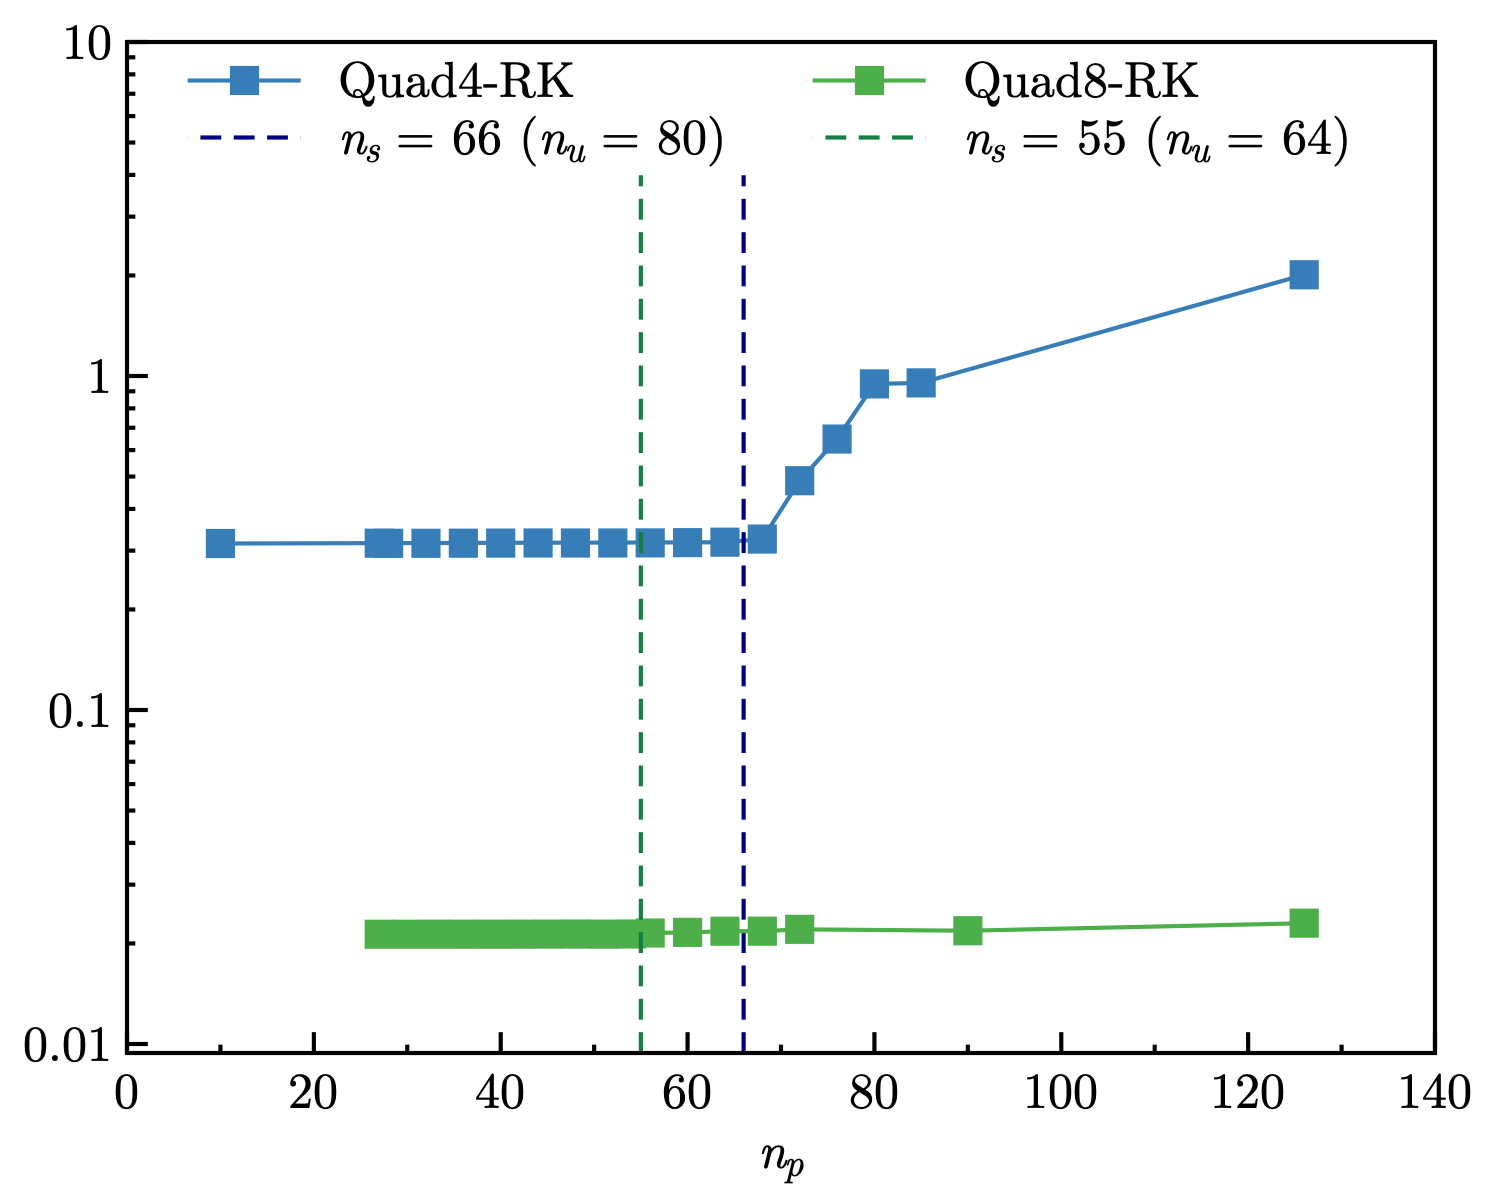
\includegraphics[width=0.48\textwidth]{cantilever_Hdev_4.png}}
& \raisebox{-0.8\height}{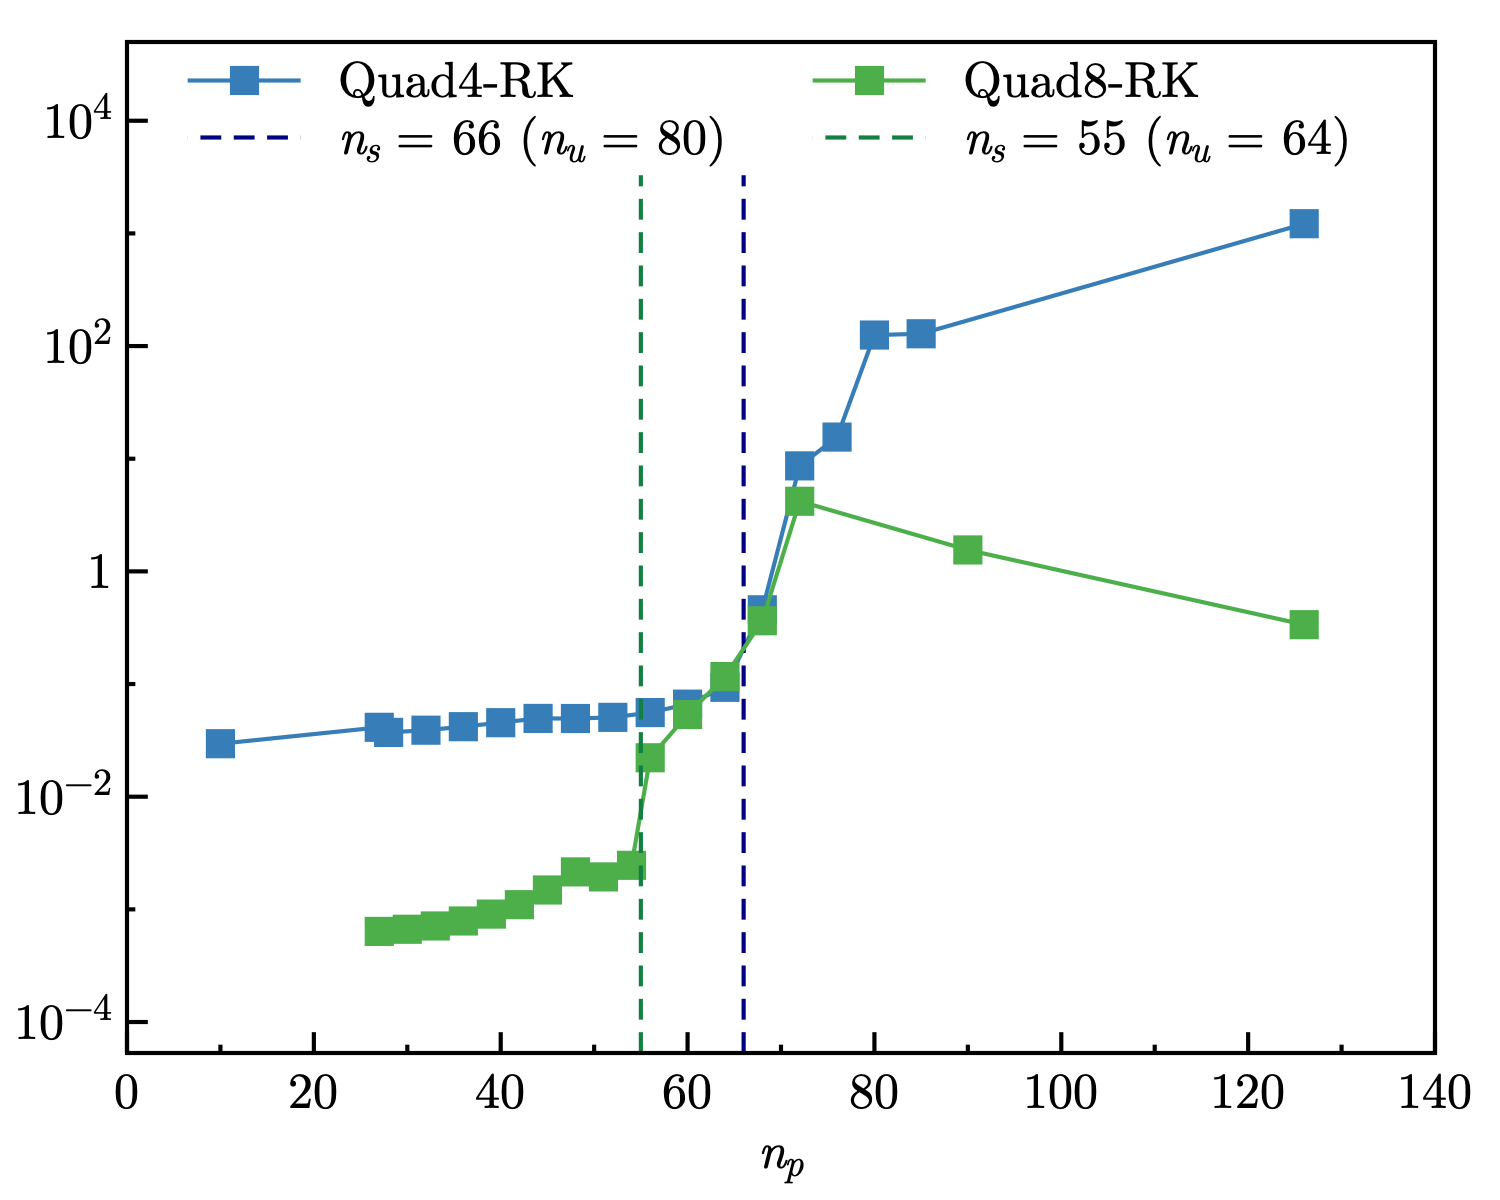
\includegraphics[width=0.48\textwidth]{cantilever_L2_p_4.png}} \\
\raisebox{-0.85\height}{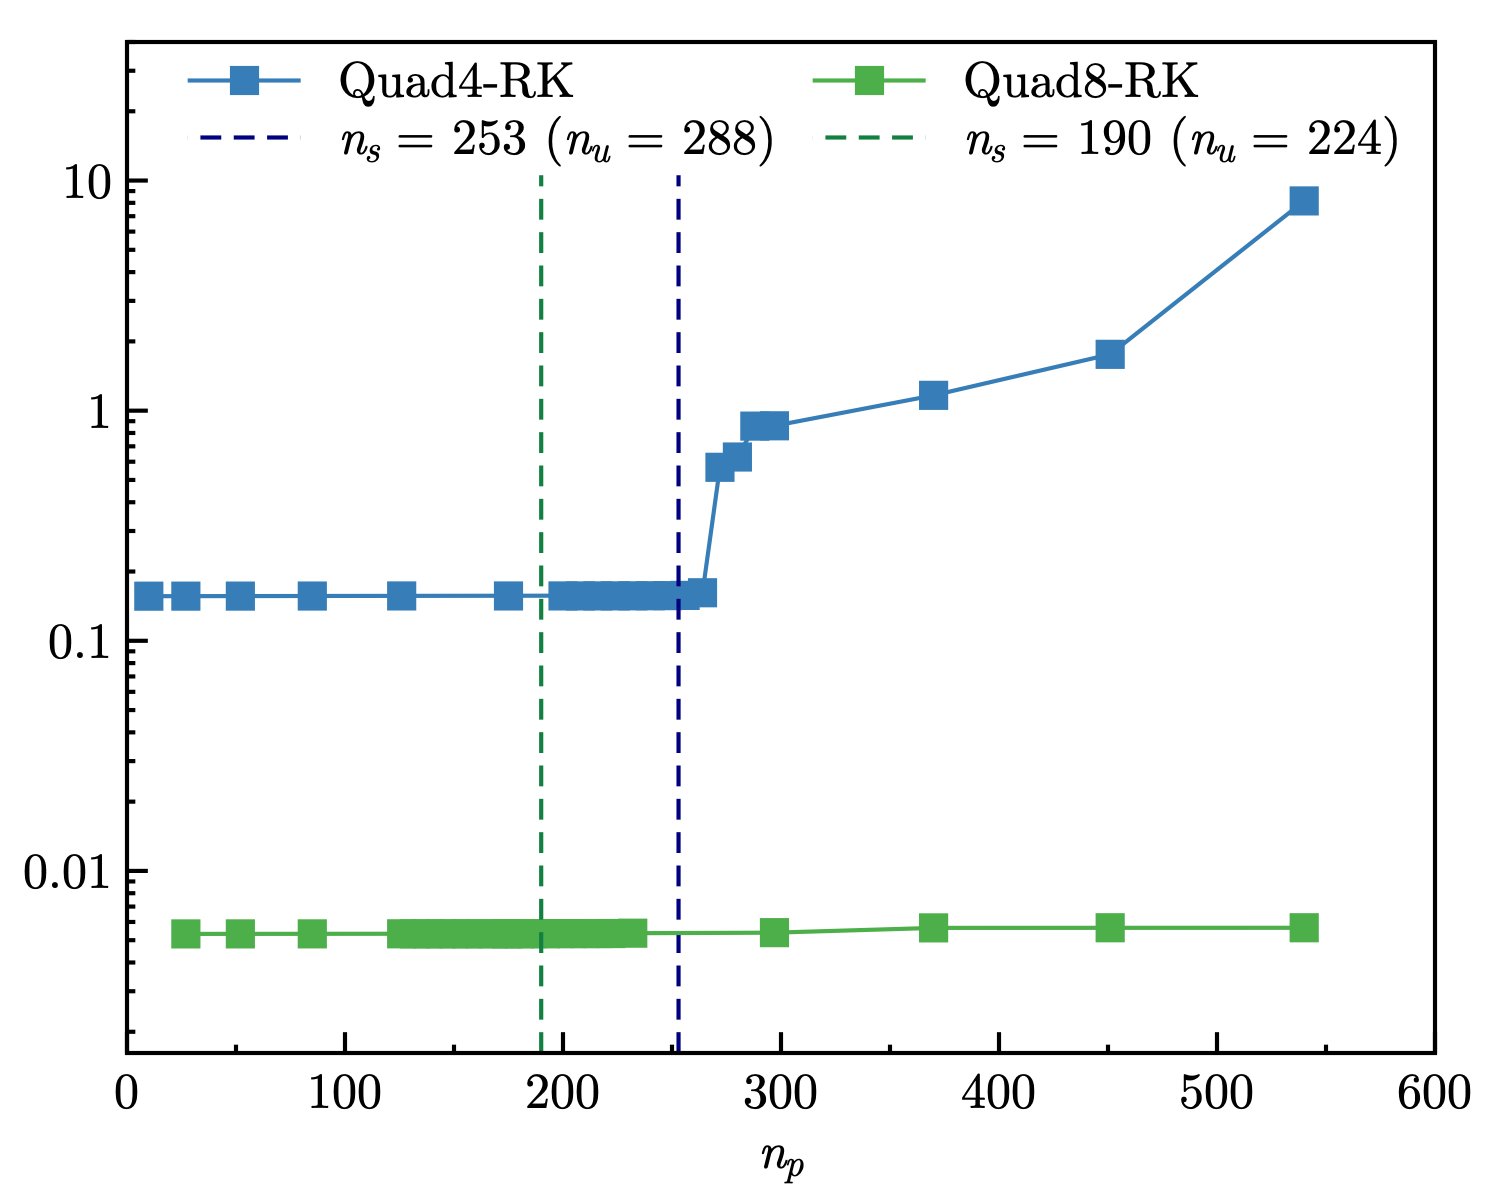
\includegraphics[width=0.48\textwidth]{cantilever_Hdev_8.png}}
& \raisebox{-0.85\height}{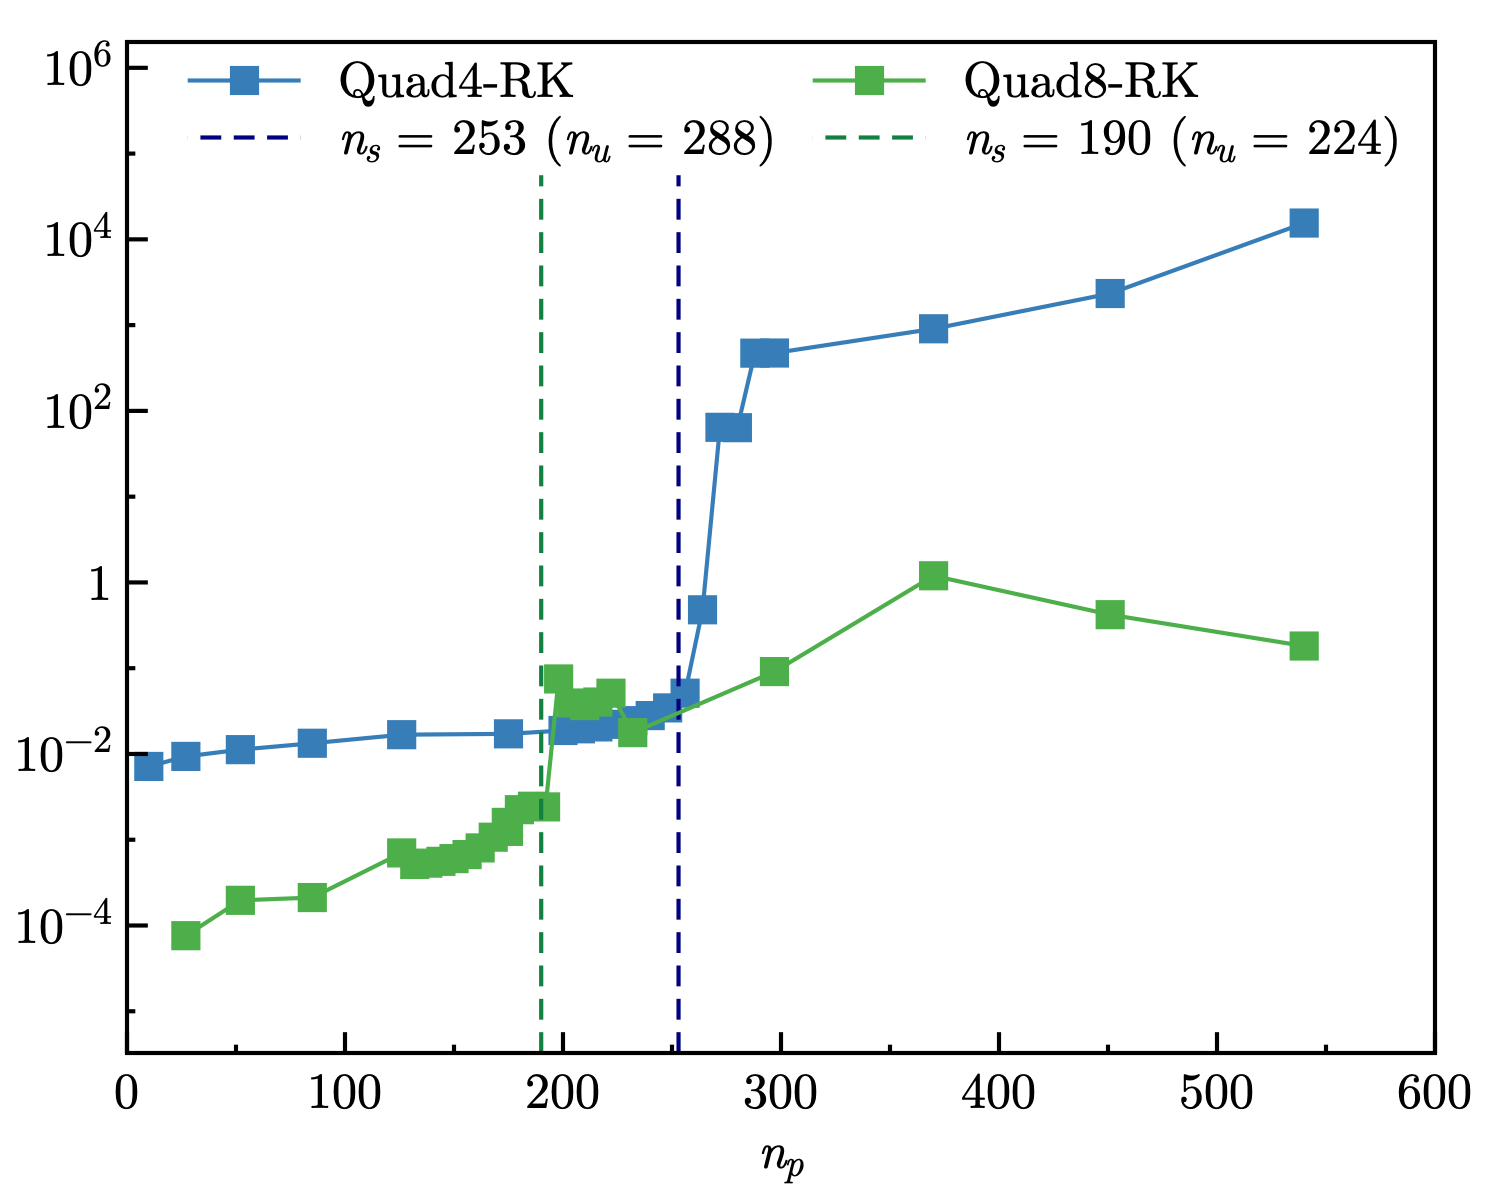
\includegraphics[width=0.48\textwidth]{cantilever_L2_p_8.png}} \\
\raisebox{-0.85\height}{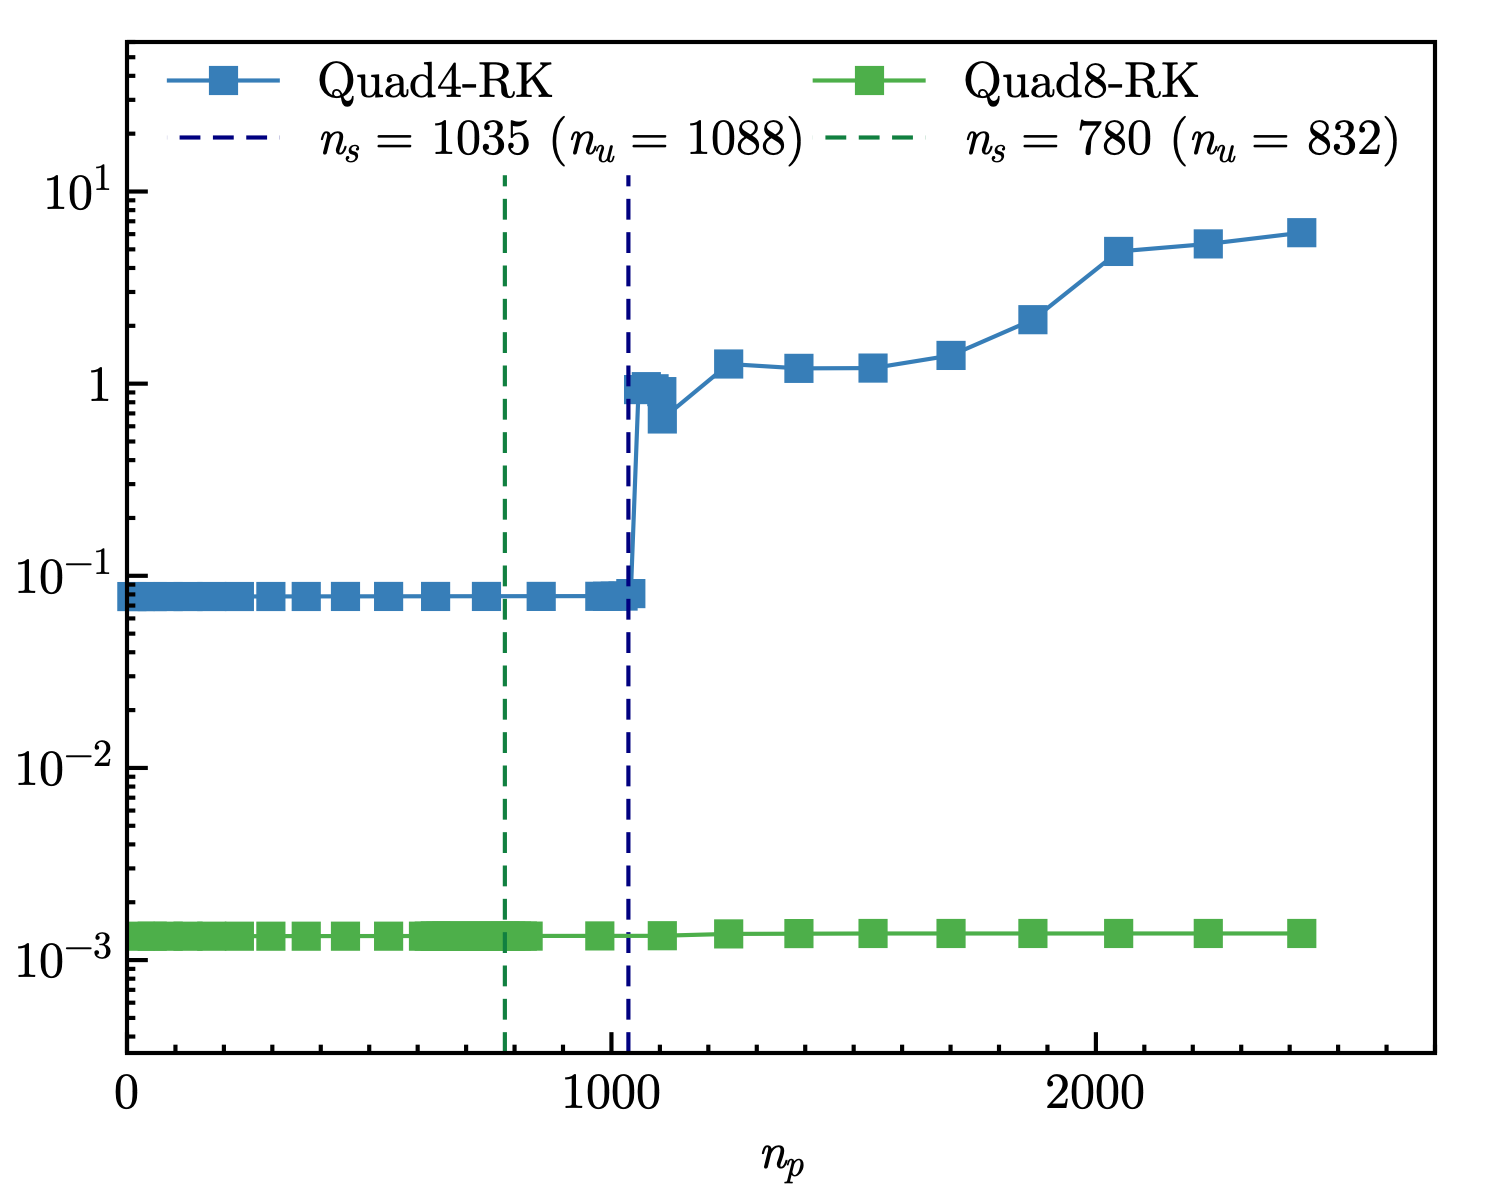
\includegraphics[width=0.48\textwidth]{cantilever_Hdev_16.png}}
& \raisebox{-0.85\height}{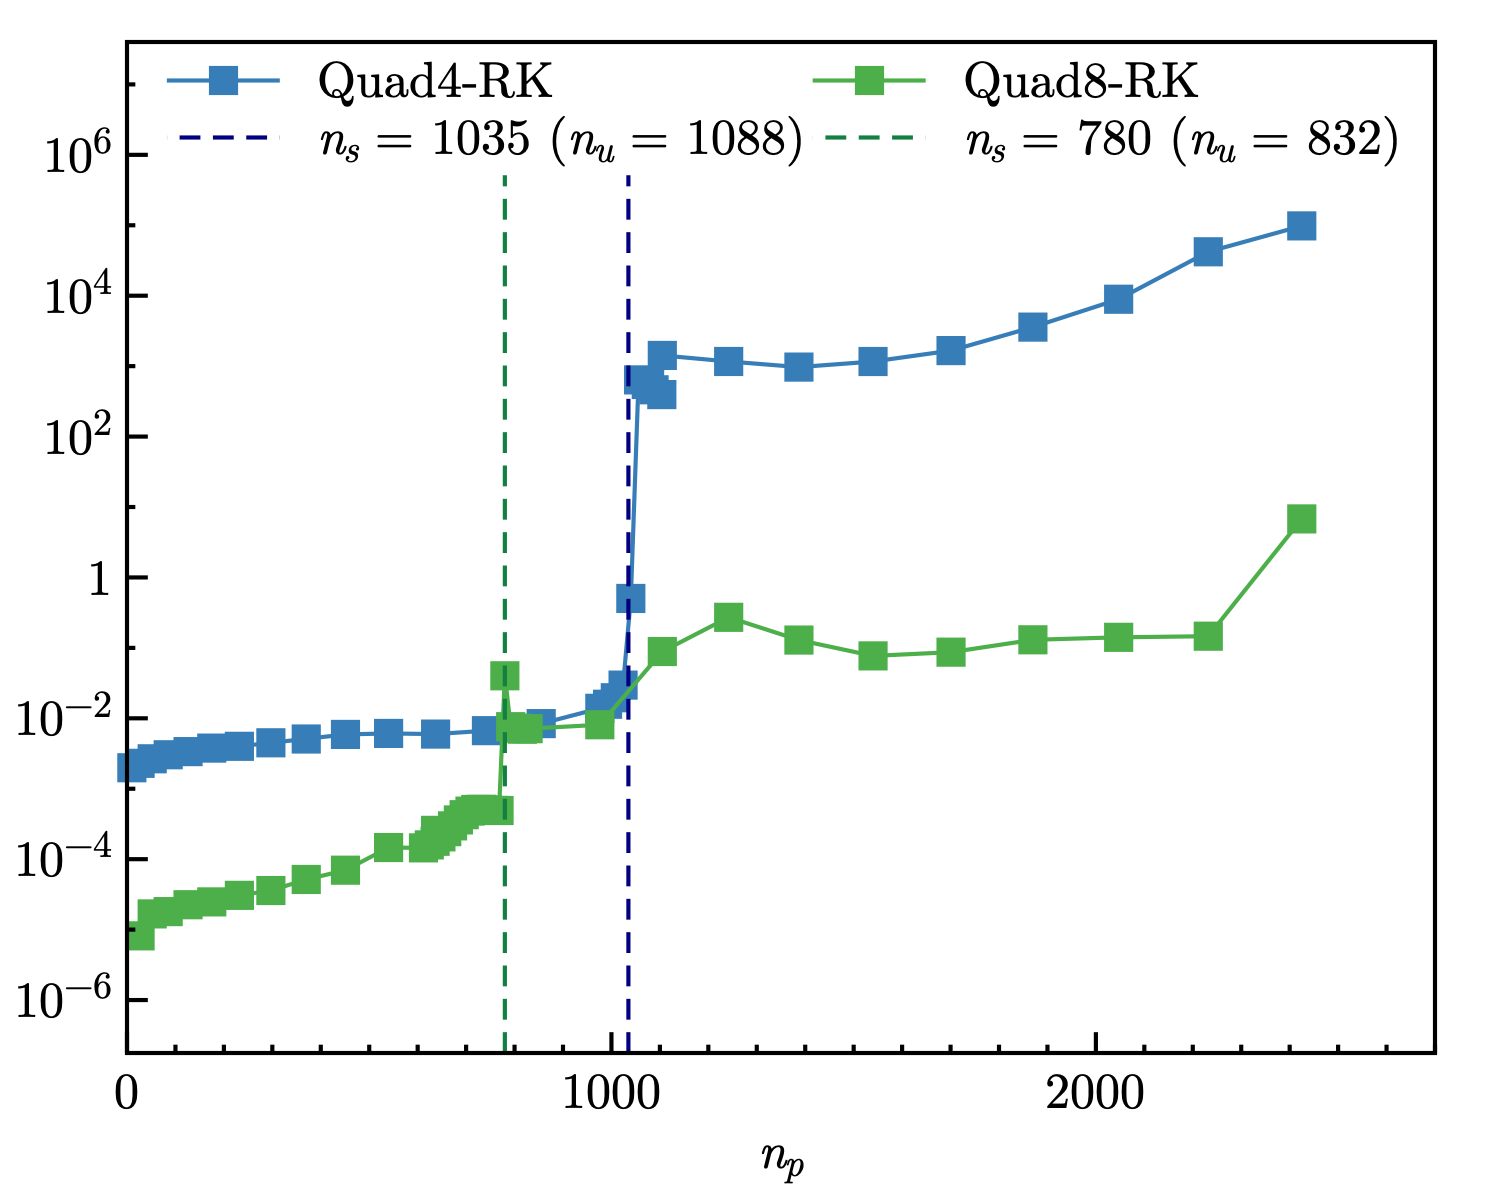
\includegraphics[width=0.48\textwidth]{cantilever_L2_p_16.png}} \\
\raisebox{-0.85\height}{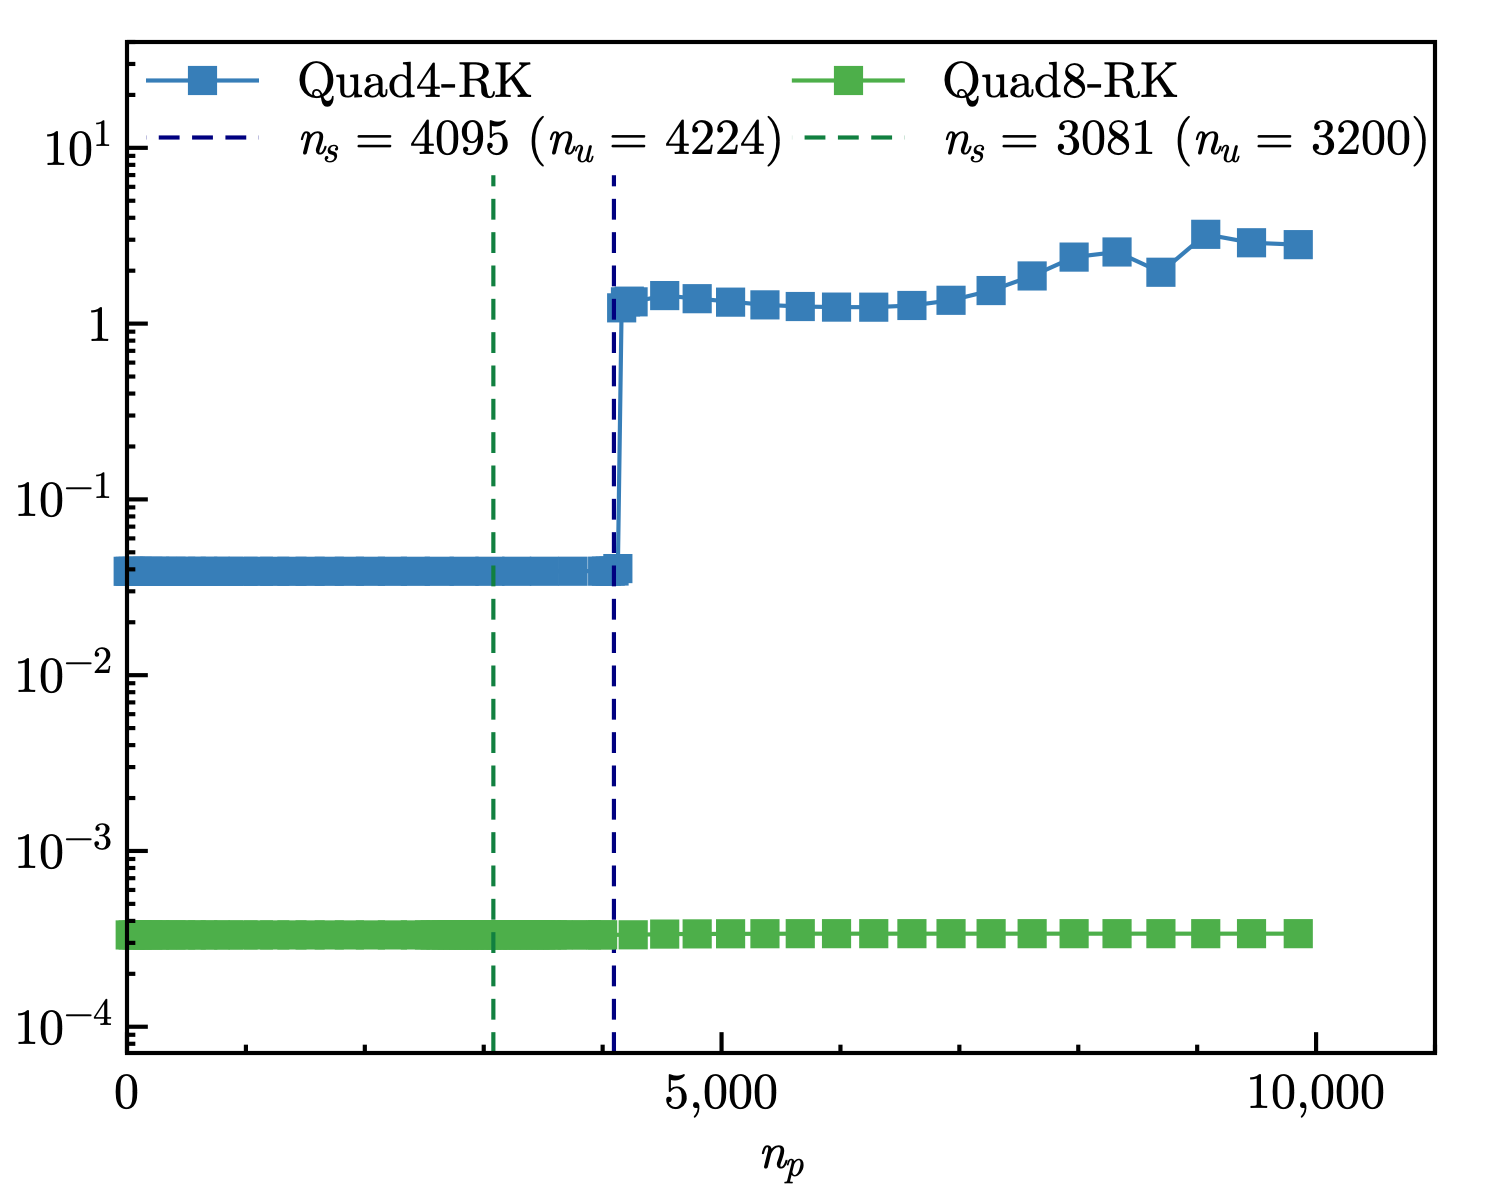
\includegraphics[width=0.48\textwidth]{cantilever_Hdev_32.png}}
 & \raisebox{-0.85\height}{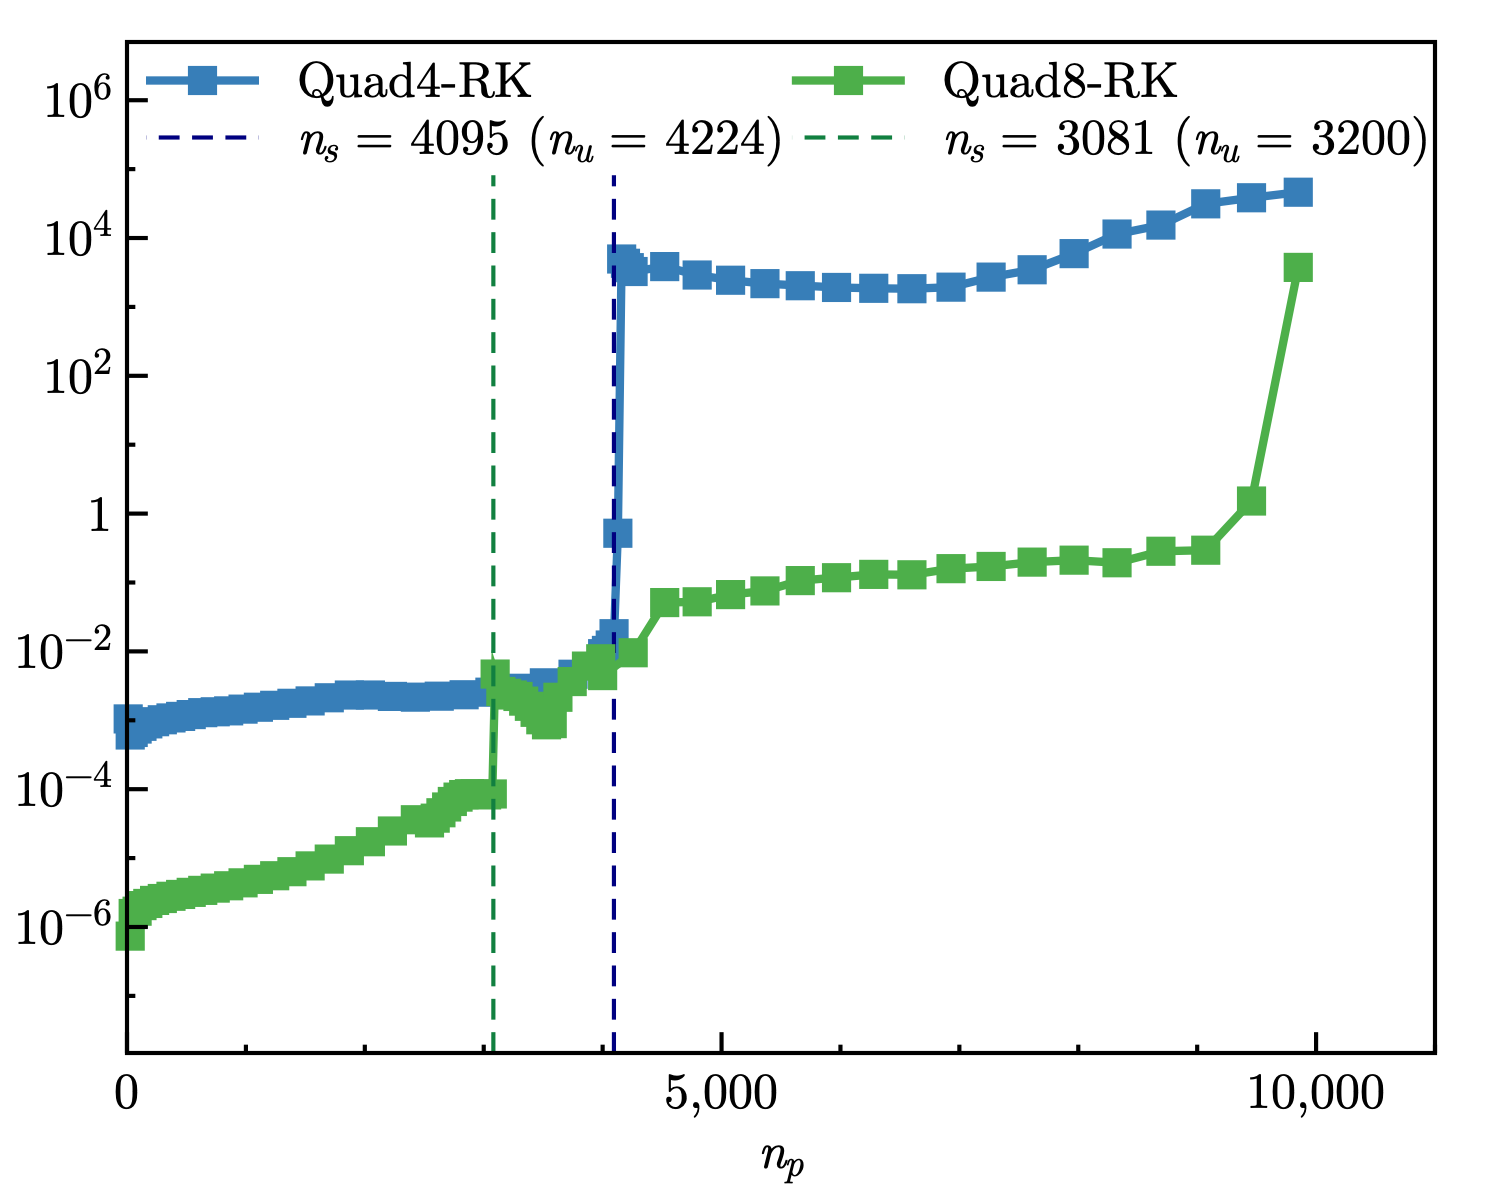
\includegraphics[width=0.48\textwidth]{cantilever_L2_p_32.png}} \\
\end{tabular}
\end{subcaptiongroup}
\caption{Strain and pressure errors vs. $n_p$ for cantilever beam problem}\label{fg:cantilever_ns}
\end{figure}

In this problem, the Quad4 element with $16\times 4$, $32\times 8$, $64\times 16$, $128\times 32$ grids, and Quad8 element with $8\times 2$, $16\times 4$, $32\times 8$, $64\times 16$ grids are employed for displacement discretization. The pressure is discretized by linear and quadratic meshfree approximations with 1.5 and 2.5 characterized support sizes respectively.
The strain and pressure errors with respect to pressure nodes $n_p$ are displayed in Figure \ref{fg:cantilever_ns}, where, to avoid the interpolation error, the pressure nodes are uniformly distributed independent with displacement nodes by the same way in Section \ref{subsec:optimal_constraint_ratio}. 
The vertical dashed lines stand for the stabilized number $n_s$. The figure implies that the Quad8 shows better performance than Quad4, since the Quad8's strain results are stable no matter the constraint ratio is in the optimal range or not. And the Quad4's displacement errors increase as soon as $n_p > n_s$. However, both Quad4's and Quad8's pressure errors immediately increase while their constraint ratios are out of the optimal range, and Quad8 still has better results than Quad4.
Figure \ref{fg:cantilever_convergence} shows the strain and pressure error convergence comparisons with Quad4--RK, Quad8--RK with $r=n_d$, $r=r_{opt}$ and traditional 4--node quadrilateral displacement element with 1--node piecewise constant pressure (Q4P1), 8--node quadrilateral displacement element with 3--node piecewise linear pressure (Q8P3) for this cantilever beam problem, in which, except Quad8--RK($r=n_d$) for strain error, all formulations with the traditional constraint ratio of $r=n_d$ cannot ensure the optimal error convergence rates. The proposed mixed formulations with $r=r_{opt}$ and Q4P1, Q8P3 can maintain the optimal error convergence ratio, except the strain error of Quad8--RK is a little larger than that of Q8P3, the proposed approaches show the best performance in accuracy.

\begin{figure}[H]
\centering
\begin{subcaptiongroup}
\centering
\parbox[b]{0.49\textwidth}{
    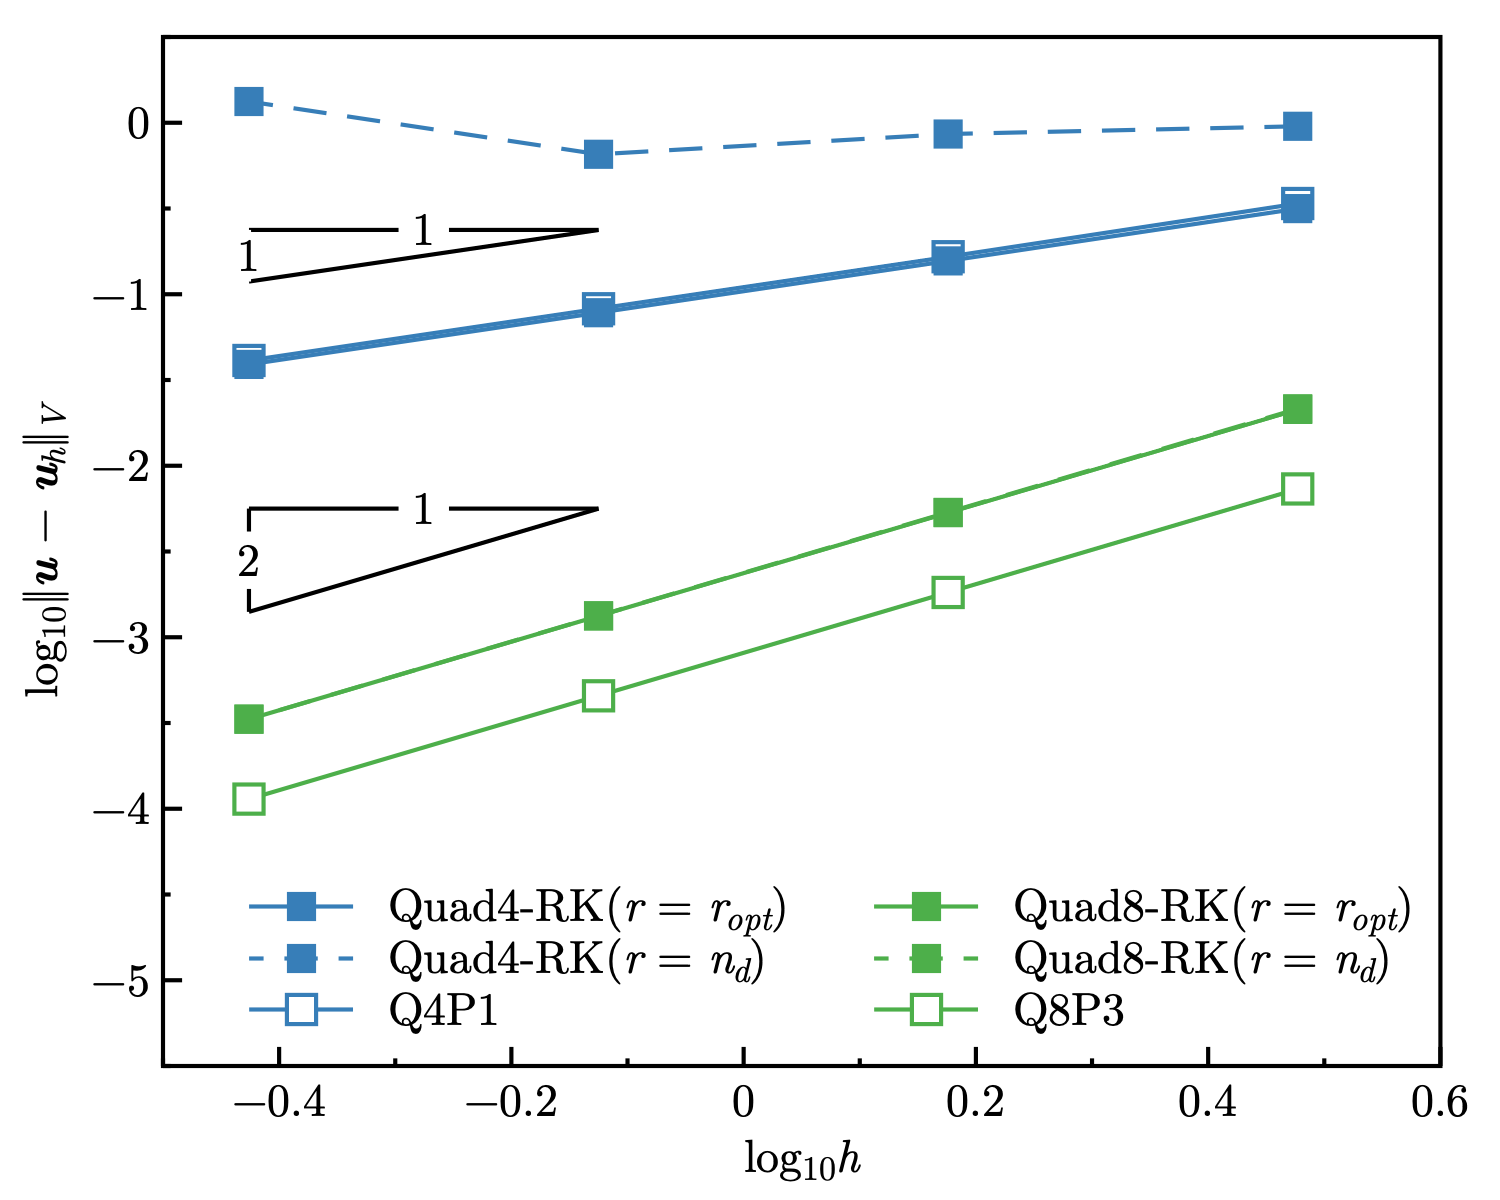
\includegraphics[width=0.49\textwidth]{cantilever_Hdev_r1.png}
    \caption{Strain error}\label{fg:cantilever_convergence_strain}
}
\parbox[b]{0.49\textwidth}{
    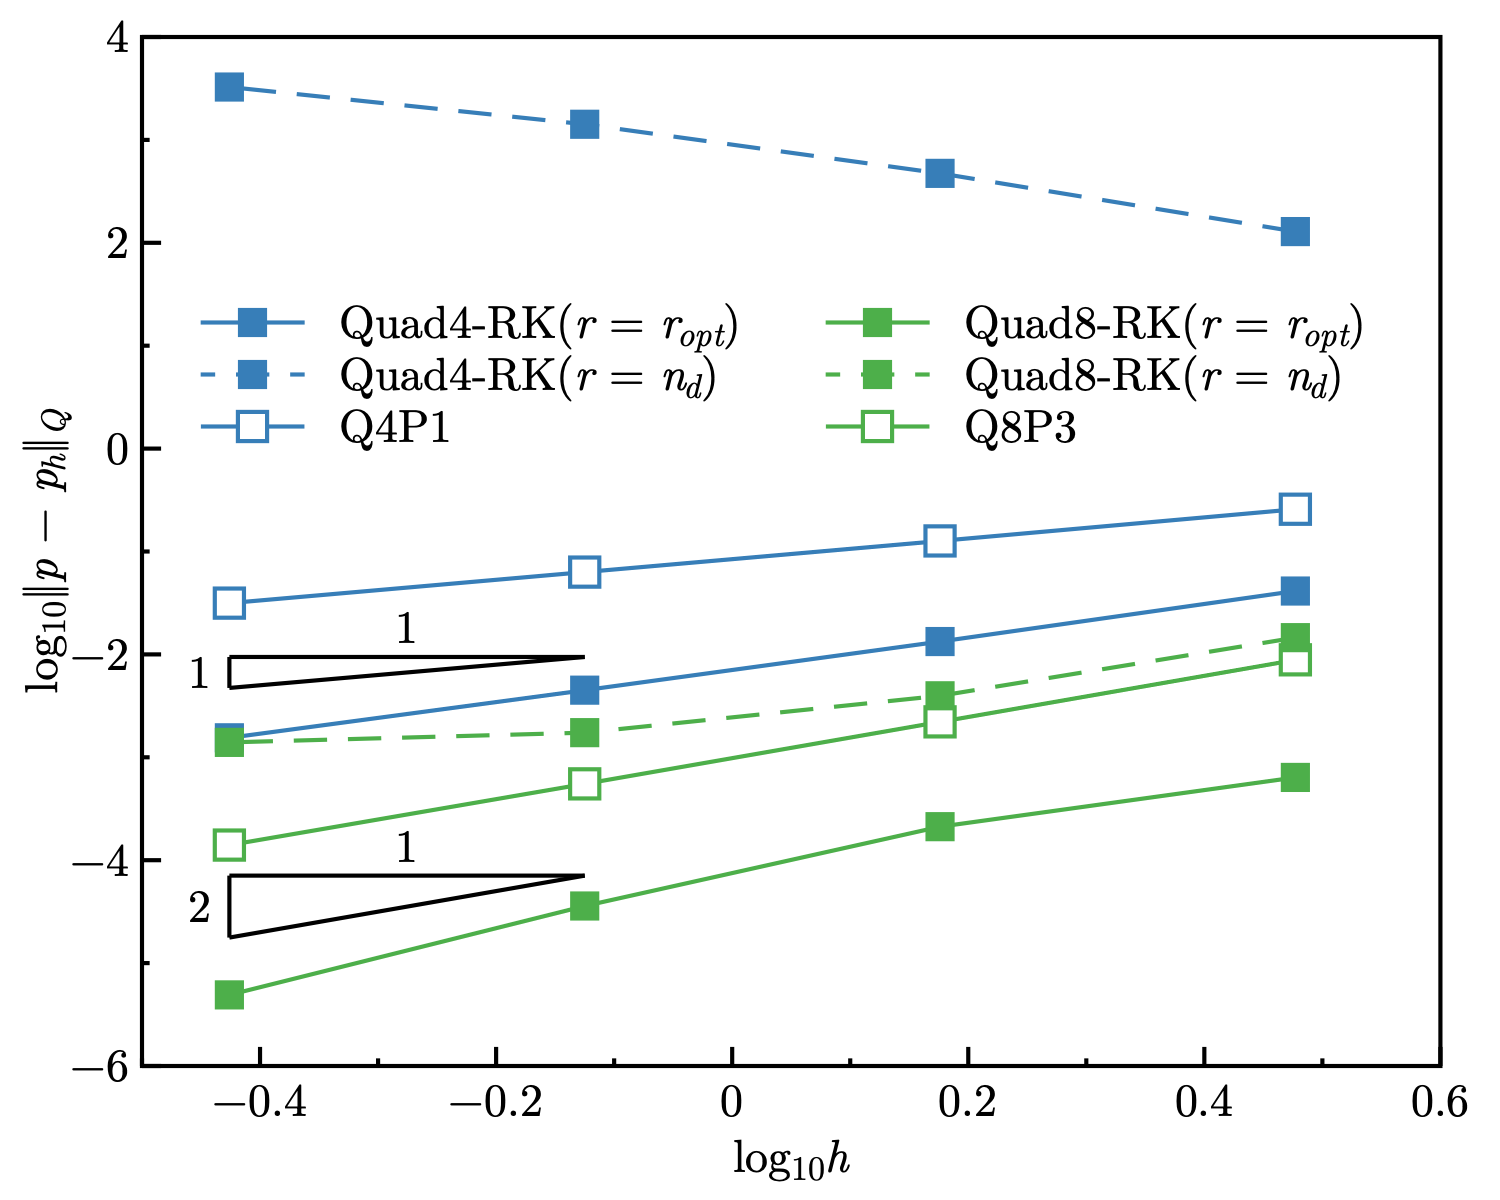
\includegraphics[width=0.49\textwidth]{cantilever_L2_p_r1.png}
    \caption{Pressure error}\label{fg:cantilever_convergence_pressure}
}
\end{subcaptiongroup}
\caption{Error convergence study for cantilever beam problem}\label{fg:cantilever_convergence}
\end{figure}

